%!TeX encoding = UTF-8 Unicode
\documentclass{article}
\usepackage[pdftex]{graphicx} %for embedding images
\usepackage{url} %for proper url entries
\usepackage[bookmarks, colorlinks=false, pdfborder={0 0 0}, pdftitle={Laboratory ML Project 01}, pdfauthor={Nhut-Nam Le}, pdfsubject={Introduction to Machine Learning}, pdfkeywords={report, exercises}]{hyperref} %for creating links in the pdf version and other additional pdf attributes, no effect on the printed document
%\usepackage[final]{pdfpages} %for embedding another pdf, remove if not required
\usepackage[utf8]{inputenc}
\usepackage[english, vietnamese]{babel}
\usepackage{float}
\usepackage{fancyhdr}
\usepackage{pythonhighlight}
\usepackage[left=3cm, right=3cm, top=2cm, bottom=2cm]{geometry}
\usepackage{parskip}
\usepackage{tikz}
\usepackage{hyperref}
\usepackage[]{algorithm2e}
\usepackage[noend]{algpseudocode}
\usepackage{amsmath}
\usepackage{amsfonts}

\usepackage{listings}
\usepackage{color}

\definecolor{dkgreen}{rgb}{0,0.6,0}
\definecolor{gray}{rgb}{0.5,0.5,0.5}
\definecolor{mauve}{rgb}{0.58,0,0.82}

\newcommand\T{\rule{0pt}{2.6ex}}       % Top strut
\newcommand\B{\rule[-1.2ex]{0pt}{0pt}} % Bottom strut


\lstset{frame=tb,
	language=Java,
	aboveskip=3mm,
	belowskip=3mm,
	showstringspaces=false,
	columns=flexible,
	basicstyle={\small\ttfamily},
	numbers=none,
	numberstyle=\tiny\color{gray},
	keywordstyle=\color{blue},
	commentstyle=\color{dkgreen},
	stringstyle=\color{mauve},
	breaklines=true,
	breakatwhitespace=true,
	tabsize=3
}

\setlength{\parindent}{15pt}
\setlength{\headheight}{15.2pt}
\pagestyle{fancy}
\lhead[<even output>]{NHẬP MÔN HỌC MÁY}
\rhead[<even output>]{BÁO CÁO ĐỒ ÁN THỰC HÀNH 01}
\title{research-outline}
\author{Nhut-Nam Le}
\date{2021}
\begin{document}
	\begin{titlepage}
		\begin{center}
			% Top of the page
			\large{\textbf{ĐẠI HỌC KHOA HỌC TỰ NHIÊN, ĐHQG-HCM\\KHOA CÔNG NGHỆ THÔNG TIN\\BỘ MÔN KHOA HỌC MÁY TÍNH}}\\
			
\includegraphics[width=0.75\textwidth]{images/khtn.png}\\
			% Title
			\large \textbf{NHẬP MÔN HỌC MÁY}\\[0.1in]
			\huge \textbf{BÁO CÁO ĐỒ ÁN THỰC HÀNH}\\[0.1in]
			\huge \textbf{REGRESSION - HỒI QUY}\\[0.1in]
			\vfill
			\normalsize
			% Submitted by
			\normalsize
			% Lecturers
			\textbf{Giảng viên lý thuyết}\\
			{\textbf{TS.} Bùi Tiến Lên}\\[0.1in]
			% Teacher Assistant
			\textbf{Giảng viên hướng dẫn}\\
			\vspace{0.1in}
			{Dương Nguyễn Thái Bảo, Nguyễn Ngọc Đức, Nguyễn Tiến Huy, Lê Thanh Phong}\\[0.1in]
			\textbf{Sinh viên thực hiện} \\
			\vspace{0.1in}
			% Submitted by
			{Vương Gia Bảo, Ngô Xuân Kiên, Lê Nhựt Nam, Nguyễn Viết Dũng}\\[0.1in]
			% Date time when written report
			\vfill
			Tháng 5 năm 2021
		\end{center}
	\end{titlepage}
	\newpage
	% End Title4
	
	\pagenumbering{roman} %numbering before main content starts
	\cleardoublepage
	%\pagebreak
	\phantomsection
	\addcontentsline{toc}{section}{Lời cảm ơn}
	\section*{Lời cảm ơn}
	\vspace{1.0in}
	\begingroup
	\setlength{\parindent}{0pt}
	\qquad Trong quá trình thực hiện đồ án này, chúng em đã nhận được rất nhiều sự giúp đỡ cũng như hỗ trợ từ các thầy cô Trường Đại học Khoa học Tự nhiên, ĐHQG-HCM và các bạn bè trong lớp Nhập môn Học Máy. Chúng em xin bày tỏ lòng cảm ơn chân thành đến mọi người vì đã giúp đỡ hướng dẫn, chỉ bảo rất tận tình.
	
	\qquad Đặc biệt, chúng em xin bày tỏ lòng biết ơn sâu sắc đến các thầy cô khoa Công nghệ Thông tin, cụ thể hơn là thầy Bùi Tiến Lên và các thầy hướng dẫn đã giảng dạy rất nhiệt, cung cấp nhiều slides, tài nguyên học tập cần thiết, tạo điều kiện tốt nhất để chúng em có thể hoàn thành được đồ án này.
	
	\qquad Trong quá trình, viết báo cáo này, chúng em không thể tránh khỏi nhiều thiếu sót, hy vọng mong nhận được góp ý từ thầy để chúng em tiếp tục hoàn thiện hơn đối với đồ án này, cũng như rút kinh nghiệm cho những đồ án, những báo cáo kế tiếp.
	
	\vspace{1.0in}
	\textbf{Đại học Khoa học Tự nhiên, ĐHQG-HCM.}\\
	Vương Gia Bảo, Ngô Xuân Kiên, Lê Nhựt Nam, Nguyễn Viết Dũng\\
	Tháng 4 năm 2021\\
	\endgroup
	
	\newpage
	\tableofcontents
	\newpage
	\pagenumbering{arabic} %reset numbering to normal for the main content
	\setcounter{secnumdepth}{0}
	
	\section{Thông tin nhóm}
	\begin{table}[H]
		\centering
		\begin{tabular}{ | p{1cm} |  p{3cm} | p{5cm} | p{5cm}  |}\hline
			STT	& MSSV & Họ tên đầy đủ & Email liên lạc \\\hline
			1 & 18120009 & Vương Gia Bảo & 18120009@student.hcmus.edu.vn  \\ \hline
			2 & 18120045 & Ngô Xuân Kiên & 18120045@student.hcmus.edu.vn \\ \hline
			3 & 18120061 & Lê Nhựt Nam & 18120061@student.hcmus.edu.vn  \\ \hline
			4 & 18120167 & Nguyễn Viết Dũng &  18120167@student.hcmus.edu.vn \\ \hline
		\end{tabular}
	\end{table}
	\section{Phân công công việc}
	\begin{table}[H]
		\begin{tabular}{ | l | l | l | p{5.5cm} | p{3cm} |}
			\hline
			STT & MSSV & Họ tên & Nội dung công việc & Mức độ hoàn thành  \\ \hline
			1 & 18120009 & Vương Gia Bảo & Thu thập dữ liệu, đọc hiểu source, báo cáo Introduction Paper &  100\%\T\B\\ \hline
			2 & 18120045 & Ngô Xuân Kiên & Thu thập dữ liệu, đọc hiểu source, báo cáo Related Work Paper & 100\%\T\B \\ \hline
			3 & 18120061 & Lê Nhựt Nam & Thu thập dữ liệu, đọc hiểu source, báo cáo, SincNet Architecture, Slides thuyết trình, Midterm Report & 100\%\T\B \\ \hline
			4 & 18120167 & Nguyễn Viết Dũng &  Thu thập dữ liệu, đọc hiểu source, báo cáo experimental setup Paper & 100\%\T\B \\ \hline
		\end{tabular}
	\end{table}
	\section{Tiêu chí đánh giá đồ án}
	\subsection{Bảng tiêu chí cho đồ án}
	\begin{table}[H]
		\begin{tabular}{ | p{5cm} | p{6.5cm} | p{3cm} |}\hline
			Tên tiêu chí đồ án & Nội dung tiêu chí & Mức độ hoàn thiện  \T\B\\\hline
			Nhận diện bài toán & Sinh viên cần tìm hiểu bài toán và dữ liệu được giao
			nhằm xác định nội dung và ý nghĩa bài toán thực tế cần giải quyết. Thông
			qua đó, sinh viên có khả năng ánh xạ vấn đề thực tế sang bài toán lập trình & 100\%  \T\B\\\hline
			Giải quyết vấn đề & Sinh viên được yêu cầu đưa ra các giải pháp và hướng
			tiếp cận nhằm giải quyết được yêu cầu bài toán thực tế & 100\%  \T\B\\\hline
			Xử lý và phân tích dữ liệu & Sinh viên có khả năng xử lý các công cụ phân
			tích dữ liệu tự động nhằm tìm ra các thông tin hữu ích, các đặc trưng tiềm ẩn
			ảnh hưởng để mục tiêu bài toán &100\%  \T\B\\\hline
			Thiết kế và cài đặt các thuật toán máy học & Sinh viên được yêu cầu có
			khả năng đề xuất, triển khai và giải thích các thuật toán máy học nhằm giải
			quyết bài toán được giao & 100\%  \T\B\\\hline
		\end{tabular}
	\end{table}
	\subsection{Bảng yêu cầu cho đồ án}
	\begin{table}[H]
		\begin{tabular}{ | p{5cm} | p{6.5cm} | p{3cm} |}\hline	
			Tên yêu cầu & Nội dung yêu cầu & Mức độ hoàn thiện  \T\B\\\hline
			Phân tích dữ liệu & Đọc và phân tích các đặc trưng trong 2 tập tin được cung cấp. Trình bày các thông tin hữu ích (insights) tác động đến chi phí y tế cá nhân & 100\%  \T\B\\\hline
			Cài đặt thuật toán & Cài đặt các thuật toán máy học đã được học để dự đoán chi phí y tế cá nhân. & 100\%  \T\B\\\hline
			Trình bày kết quả và nhận xét & Báo cáo kết quả đạt được sau quá trình phân tích và cài đặt. Từ đó nhận xét về các tác nhân ảnh hưởng mạnh/yếu tới chi phí y tế cá nhân & 100\%  \T\B\\\hline
		\end{tabular}
	\end{table}	
	\subsection{Bảng danh sách các thuật toán Hồi quy}
	\begin{table}[H]
		\begin{tabular}{ | p{3cm} | p{5cm} | p{3cm} | p{3cm} |} \hline	
			Thuật toán máy học & Cách cài đặt & Thư viện để đối chiếu (Nếu có) & Đánh giá hoàn thành\T\B\\\hline
			Multi Linear Regression & & & 100\%  \T\B\\\hline
			Logistic Regression & & & 100\%  \T\B\\\hline
			Ridge Regression & & & 100\%  \T\B\\\hline
			Lasso Regression & & & 100\%  \T\B\\\hline
			Random Forest Regressor & & & 100\%  \T\B\\\hline
			Polynomial Regression & & & 100\%  \T\B\\\hline
		\end{tabular}
	\end{table}		
	\section{Nội dung báo cáo}
	
	\section{1. Đọc dữ liệu}
	\qquad Để cho thuận tiện trong quá trình demo trên môi trường \textbf{Google Colab} nhóm chúng em sử dụng lệnh wget trên Linux, dowload trực tiếp dữ liệu từ đường dẫn mà thầy đã public trong bài lab này.
	\begin{figure}[H]
		\centering
		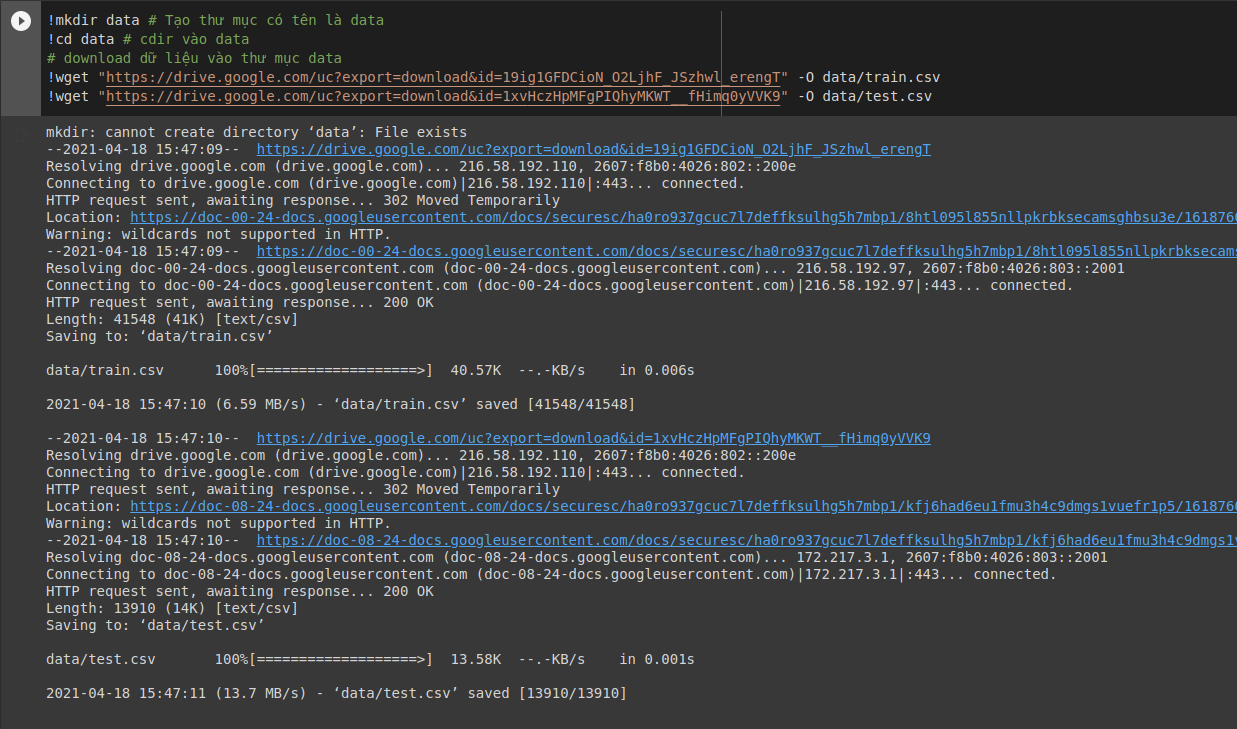
\includegraphics[width=1\textwidth]{images/download_data.png}
		\caption{Download dữ liệu: train data, test data}
		\label{fig:writing-thesis-dowload-data}
	\end{figure}
	
	Phần import một số thư viện cần thiết cho việc nhập xuất dữ liệu, xử lý dữ liệu dạng bảng, trực quan hóa dữ liệu, thư viện cung cấp các mô hình máy học
	\begin{figure}[H]
		\centering
		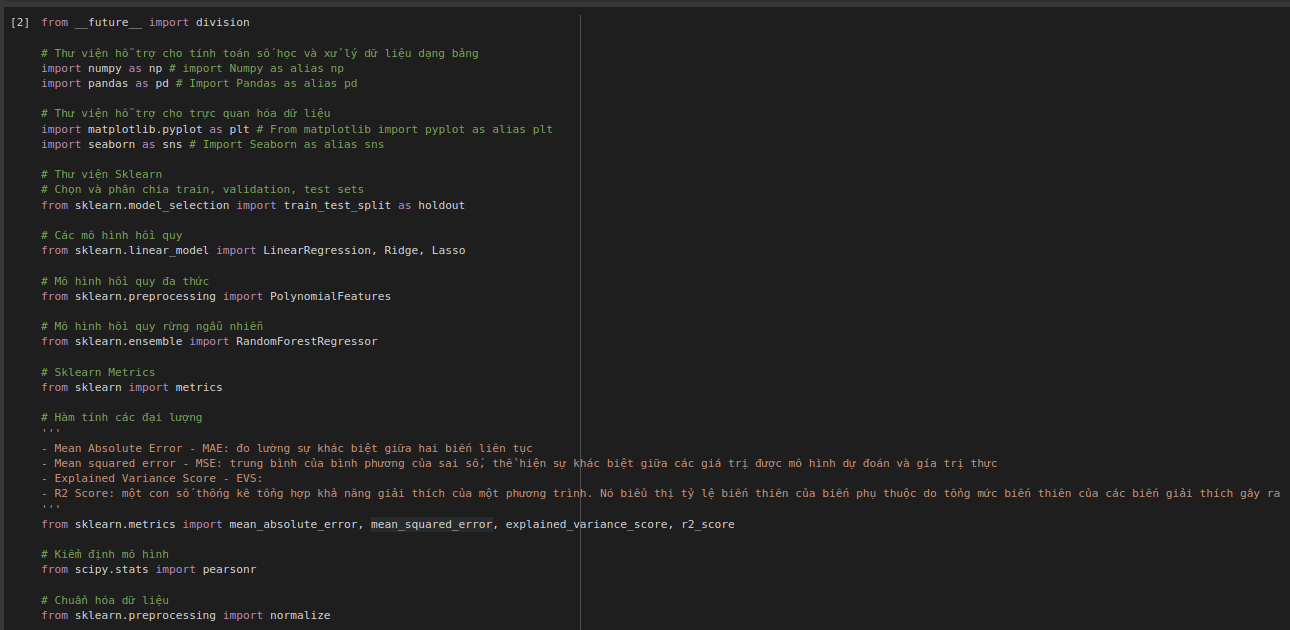
\includegraphics[width=1\textwidth]{images/import_section.png}
		\caption{Import các thư viện hỗ trợ}
		\label{fig:writing-thesis-import-section}
	\end{figure}
	
	Phần đọc dữ liệu, sử dụng thư viện Pandas như sau
	\begin{figure}[H]
		\centering
		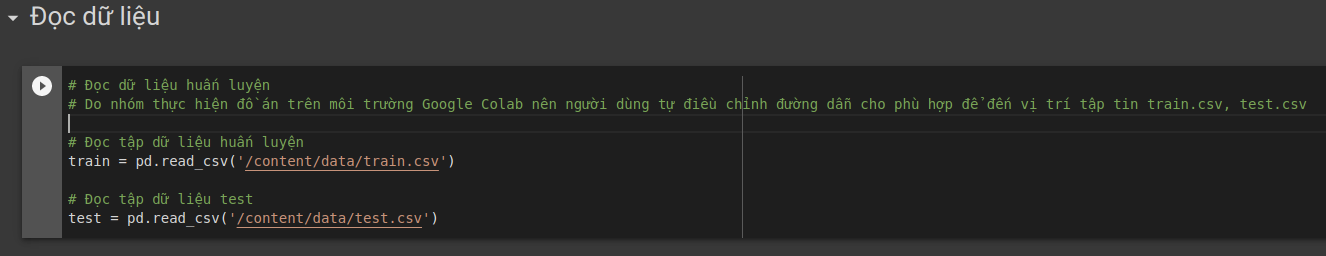
\includegraphics[width=1\textwidth]{images/read_train_test.png}
		\caption{Đọc dữ liệu}
		\label{fig:writing-thesis-read-train-test-data}
	\end{figure}
	
	\section{2. Phân tích dữ liệu}
	
	\subsection{1. Tổng quan dữ liệu thông qua các đại lượng thống kê cơ bản}
	\begin{figure}[H]
		\centering
		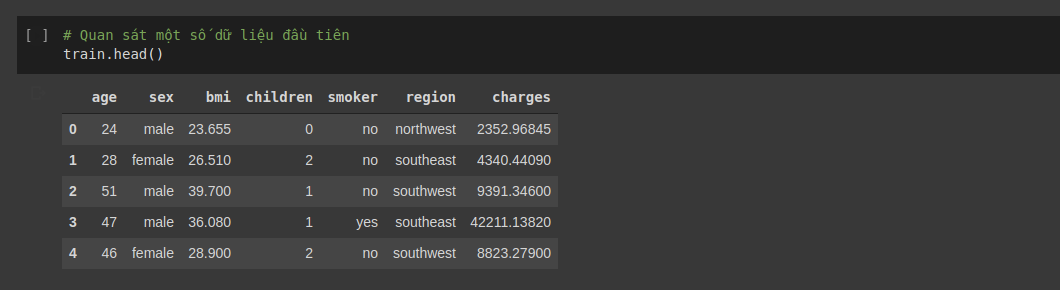
\includegraphics[width=1\textwidth]{images/train_head.png}
		\caption{Hiển thị một phần dữ liệu huấn luyện đầu tiên}
		\label{fig:writing-thesis-train-head}
	\end{figure}
	
	\subsection{2. Các đại lượng thống kê cơ bản của đặc trưng chi phí y tế}
	\begin{figure}[H]
		\centering
		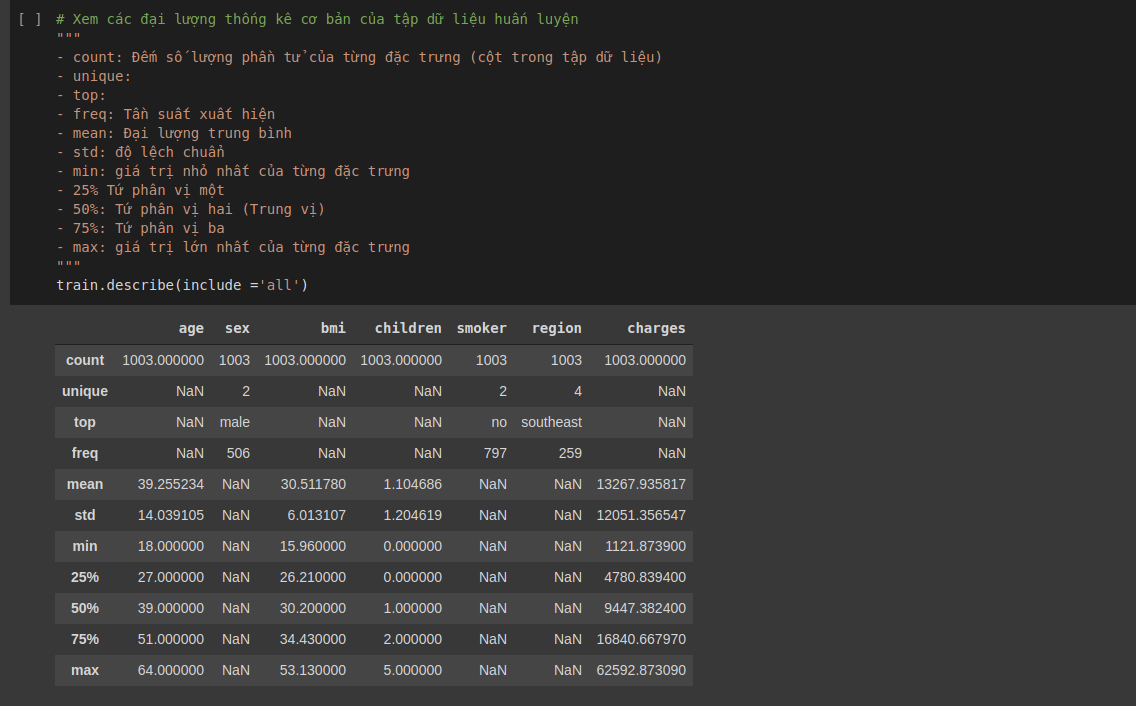
\includegraphics[width=1\textwidth]{images/simple_stat_on_train_set.png}
		\caption{Thống kê mô tả trên tập huấn luyện}
		\label{fig:writing-thesis-simple-stat-on-train-set}
	\end{figure}

	\begin{figure}[H]
		\centering
		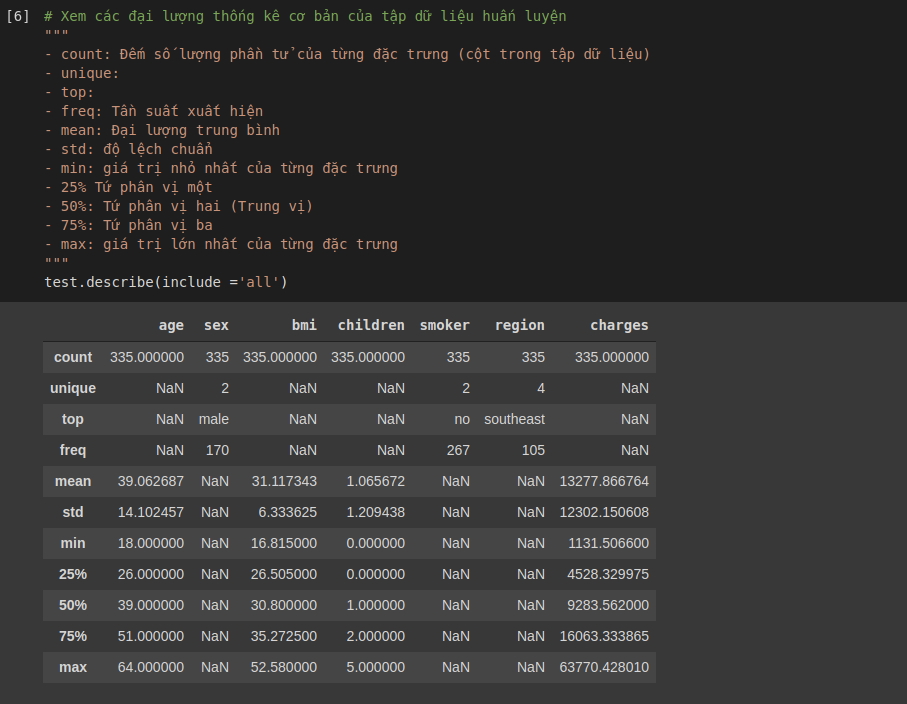
\includegraphics[width=1\textwidth]{images/simple_stat_on_test_set.png}
		\caption{Thống kê mô tả trên tập kiểm tra}
		\label{fig:writing-thesis-simple-stat-on-test-set}
	\end{figure}

	\begin{figure}[H]
		\centering
		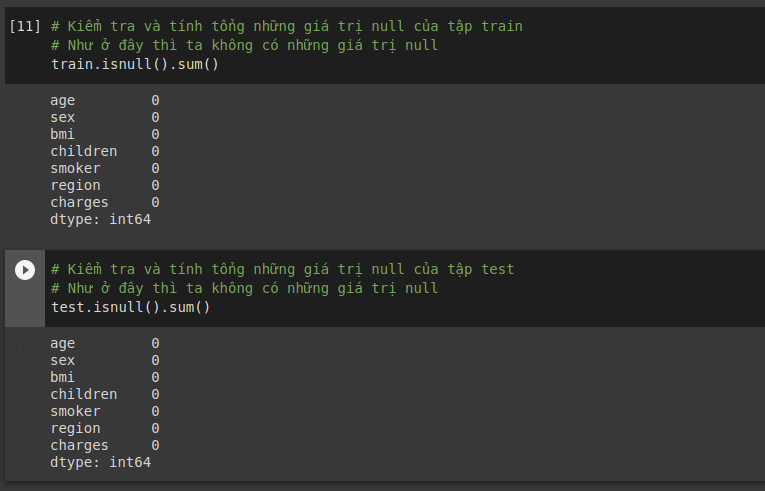
\includegraphics[width=1\textwidth]{images/check_null_train_test.png}
		\caption{Kiểm tra null values trên hai tập: tập huấn luyện, tập kiểm tra}
		\label{fig:writing-thesis-check-null-train-test}
	\end{figure}

	\begin{figure}[H]
		\centering
		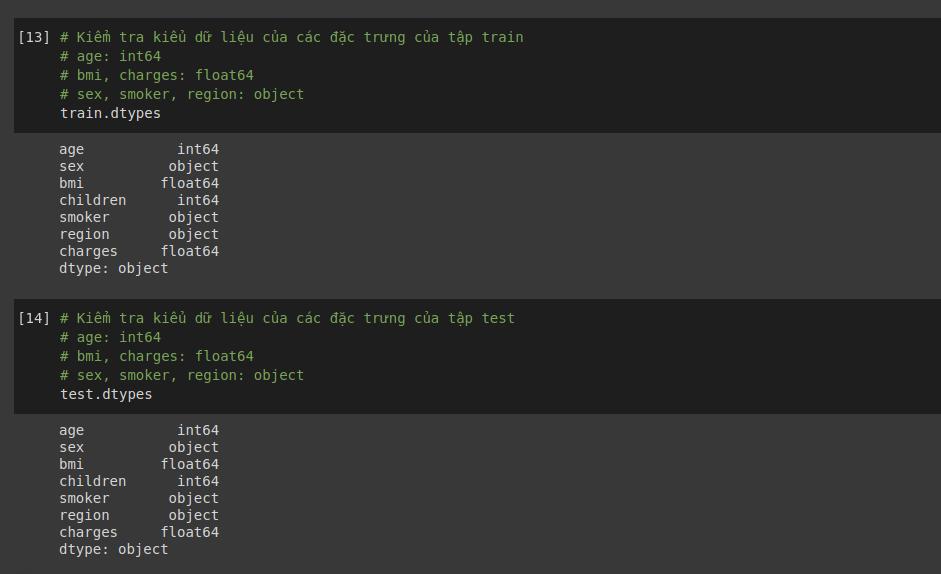
\includegraphics[width=1\textwidth]{images/data_types_train_test.png}
		\caption{Kiểm tra kiểu dữ liệu trên hai tập: tập huấn luyện, tập kiểm tra}
		\label{fig:writing-thesis-data-type-train-test}
	\end{figure}

	
	\subsection{3. Mối tương quan giữa các đặc trưng trong dữ liệu}
	\begin{figure}[H]
		\centering
		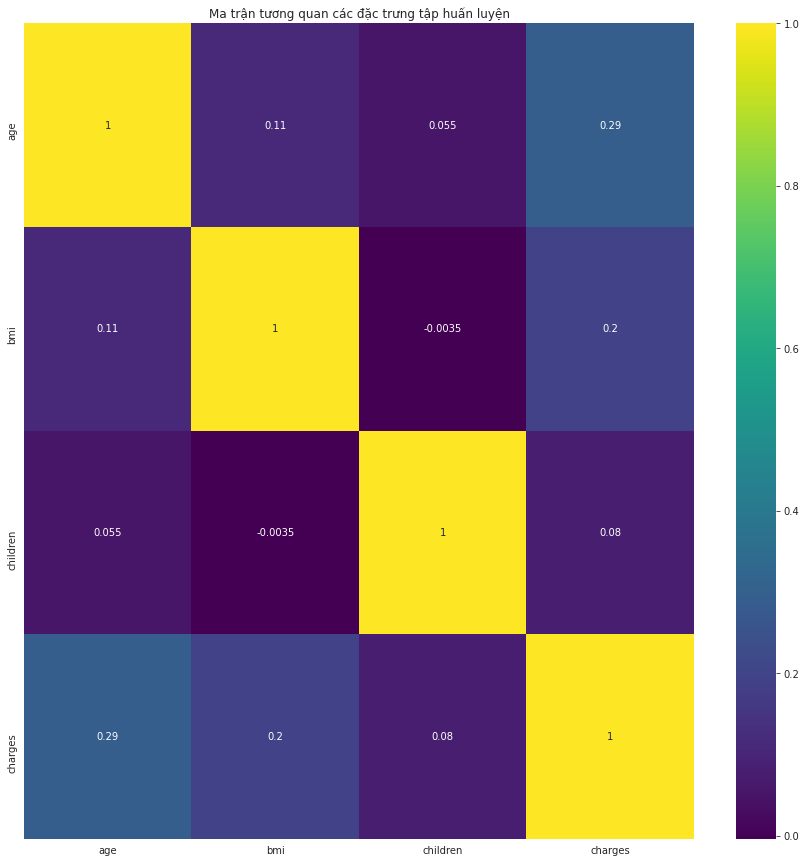
\includegraphics[width=0.7\textwidth]{images/corr_matrix_train.png}
		\caption{Ma trận tương quan giữa các đặc trưng trong tập huấn luyện}
		\label{fig:writing-thesis-corr-matrix-train}
	\end{figure}
	
	\begin{figure}[H]
		\centering
		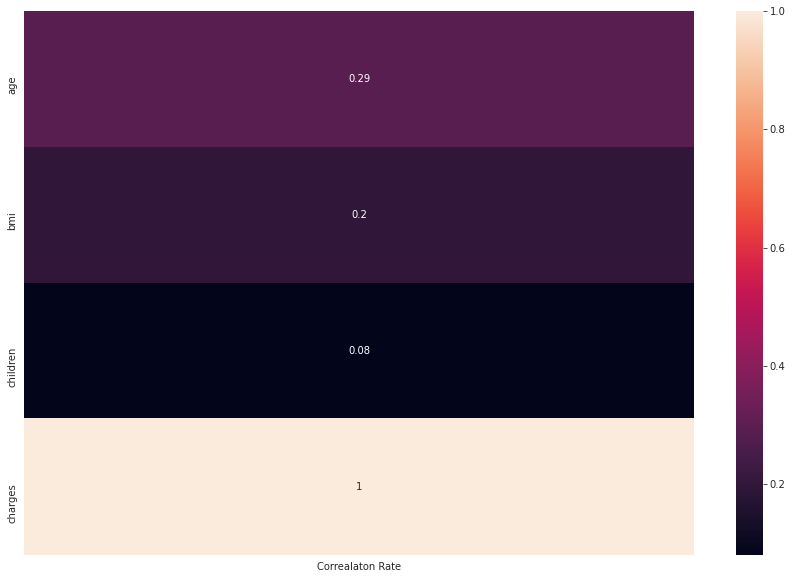
\includegraphics[width=0.7\textwidth]{images/corr_charges_other_features.png}
		\caption{Ma trận tương quan giữa chi phi y tế với các đặc trưng trong tập huấn luyện}
		\label{fig:writing-thesis-corr-charges-other-features}
	\end{figure}
	\textbf{Nhận xét:} Giữa các cặp đặc trưng dữ liệu có mối quan hệ tương đối thấp, hệ số tương quan giữa chúng bé hơn 0.5. Điều này chúng ta cần suy đoán, cần phải thêm một số điều kiện khác nữa để rút ra mối quan hệ giữa chúng với chi phí y tế: vùng (Region), tình trạng hút thuốc (Smoker) và số lượng trẻ con/ người phụ thuộc (children)
	
	\subsection{4. Phân tích đặc trưng chi phí y tế}
	\begin{figure}[H]
		\centering
		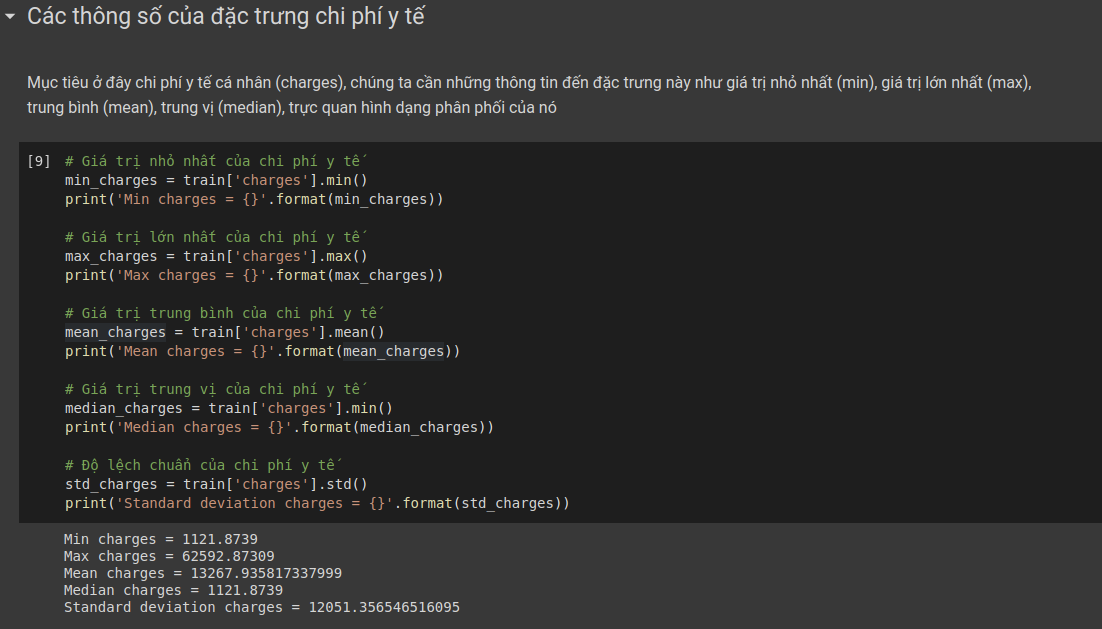
\includegraphics[width=1\textwidth]{images/medical_charges.png}
		\caption{Thông số thống kê cơ bản về đặc trưng chi phí y tế}
		\label{fig:writing-thesis-medical-charges}
	\end{figure}
	Một số thống kê cơ bản về chi phí y tế:
	\begin{itemize}
		\item  Chi phí thấp nhất của chi phí y tế - Min charges = 1121.8739
		\item  Chi phí cao nhất của chi phí y tế - Max charges = 62592.87309
		\item  Chi phí trung bình của chi phí y tế - Mean charges = 13267.935817337999
		\item  Giá trị trung vị của chi phí y tế- Median charges = 1121.8739
		\item  Độ lệch chuẩn của chi phí y tế - Standard deviation charges = 12051.356546516095
	\end{itemize}
	Trực quan phân phối của đặc trưng chi phí y tế: Dùng displot seaborn để trực quan phân phối của đặc trưng y tế
	\begin{figure}[H]
		\centering
		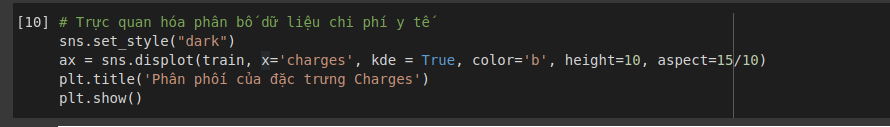
\includegraphics[width=1\textwidth]{images/dist_medical_charges.png}
		\caption{Dùng displot Seaborn để trực quan phân phối của đặc trưng chi phí y tế}
		\label{fig:writing-thesis-dist-medical-charges}
	\end{figure}
	
	\begin{figure}[H]
		\centering
		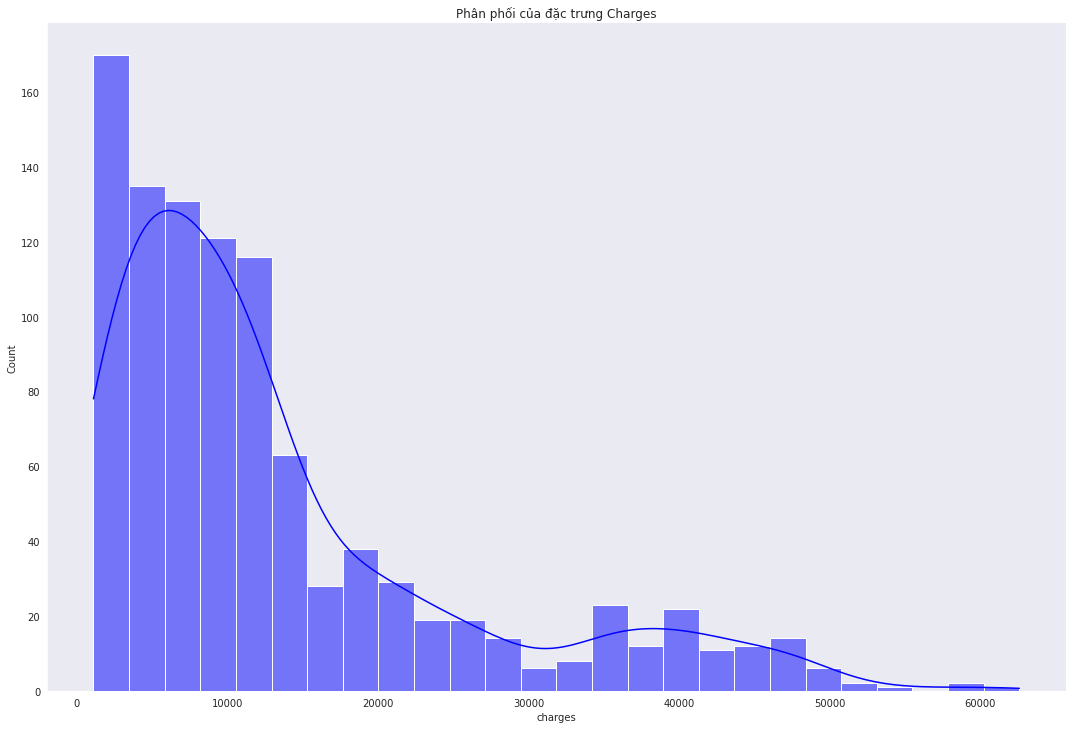
\includegraphics[width=1\textwidth]{images/dist_medical_charges_plot.png}
		\caption{Dùng displot Seaborn để trực quan phân phối của đặc trưng chi phí y tế}
		\label{fig:writing-thesis-dist-medical-charges-plot}
	\end{figure}
	\textbf{Nhận xét:} Chi phí trung bình của chi phí y tế lớn hơn rất nhiều so với Giá trị trung vị của chi phí y tế dẫn đến phân phối bị lệch sang một phía (sang trái), hình dạng phân phối này không gần phần phối chuẩn, ta có thể dùng Numpy log để tính và vẽ lại biểu dô. Hàm log và f(x) đồng biến nên sẽ không mất tính tổng quát khi xem xét phân phối của dữ liệu hay đặc trưng.

	\begin{figure}[H]
		\centering
		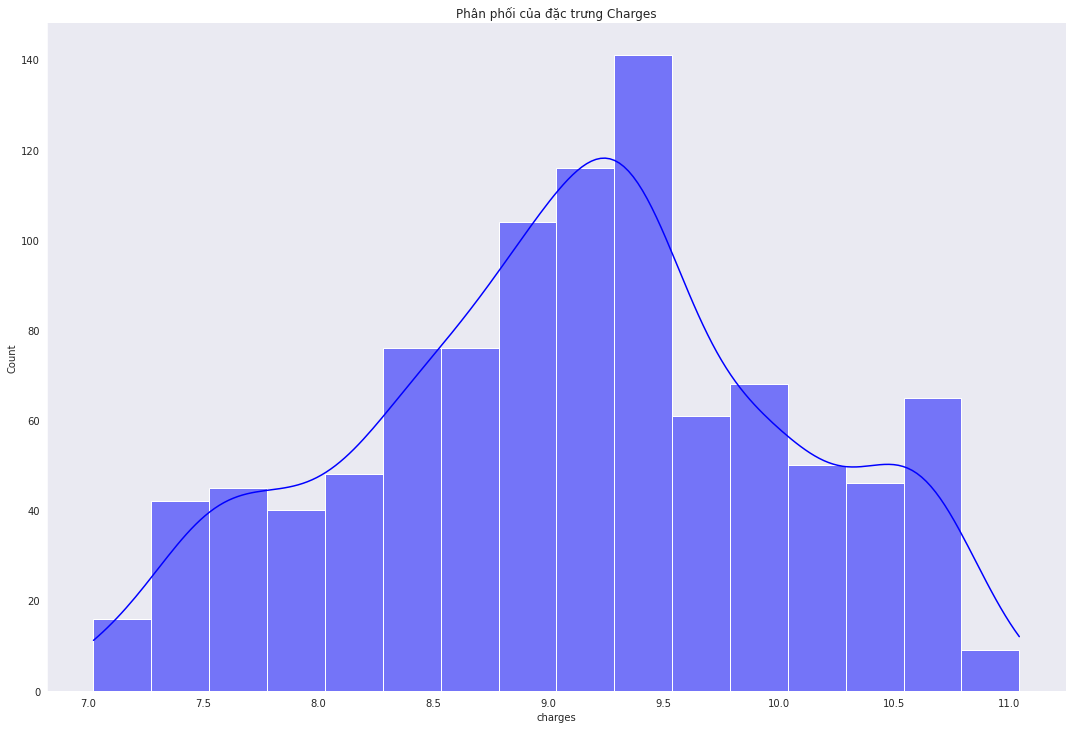
\includegraphics[width=1\textwidth]{images/dist_medical_charges_plot_log_scale.png}
		\caption{Dùng displot Seaborn để trực quan phân phối của đặc trưng chi phí y tế}
		\label{fig:writing-thesis-dist-medical-charges-plot-log-scale}
	\end{figure}
	\textbf{Nhận xét:} Hình dạng sau khi áp dụng Numpy Log, đặc trưng chi phí y tế có dạng của phân phối chuẩn, điều này cho thấy dữ liệu không có điểm bất thường.
	
	\subsection{4. Phân tích mối quan hệ chi phí y tế (charges) - vùng (region)}
	\qquad Do các giá trị trên ma trận tương quan tương đối nhỏ đối với cặp đặc trưng, nên nhóm quyết định chuyển hướng suy luận thông qua việc xem xét nhiều đặc trưng.
	
	Ở phần này, nhóm phân tích mối quan hệ giữa chi phí y tế (charges) và vùng (region)
	
	Theo như dữ liệu phía trên, đặc trưng region có 4 giá trị:
	\begin{itemize}
		\item northwest - vùng Tây Bắc
		\item northeast - vùng Đông Bắc
		\item southeast - vùng Đông Nam
		\item southwest - Vùng Tây Nam
	\end{itemize}
	Nhóm sử dụng biểu đồ cột để trực quan quá tổng giá trị chi phí ở từng vùng trên.
	\begin{figure}[H]
		\centering
		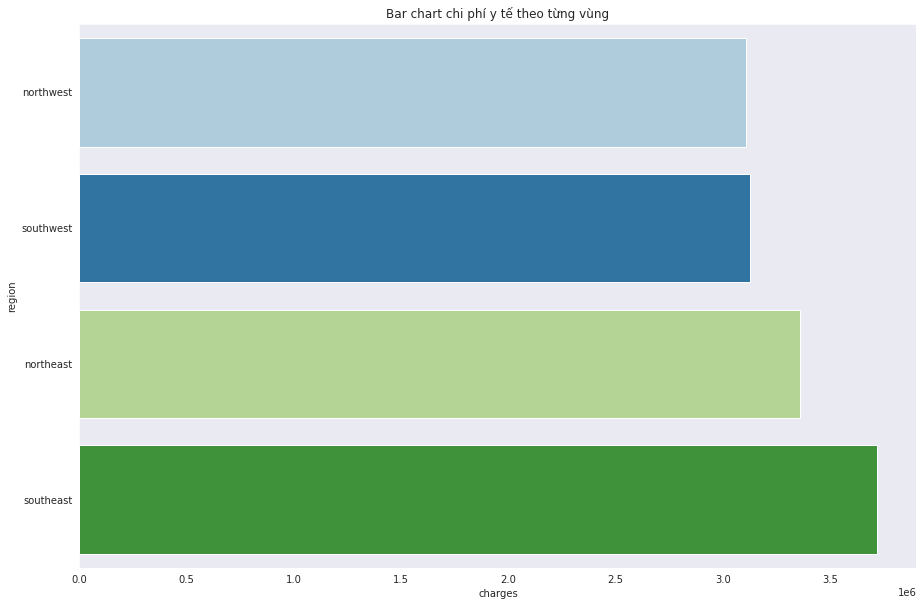
\includegraphics[width=1\textwidth]{images/bar_chart_medical_charges_region.png}
		\caption{Chi phí y tế theo từng vùng}
		\label{fig:writing-thesis-bar-chart-medical-charges-region}
	\end{figure}
	\textbf{Nhận xét:} 
	\begin{itemize}
		\item 	Biểu đồ thể hiện chi phí y tế theo từng vùng. Chúng ta có 4 vùng cần xem xét: Northwest (vùng Đông Bắc), Southwest (vùng Tây Bắc), Northeast (vùng Tây Nam) và Southeast (vùng Đông Nam). Trong đó, vùng Tây Nam là vùng có chi phí y tế cao nhất, hai vùng Đông Bắc và Tây Bắc có chi phí y tế thấp hơn các vùng còn lại.
		\item Ngoài ra, nếu chia thành 2 phần Tây và Đông thì cư dân ở vùng phía Đông (Đông Bắc, Đông Nam) có chi phí khá cao so với cư dân ở vùng phía Tây (Tây Bắc, Tây Nam) bên kia.
		\item Nhóm nhận định rằng đặc trưng \textbf{vùng} có ít ảnh hưởng đến chi phí y tế cá nhân.
	\end{itemize}

	\subsection{5. Phân tích mối quan hệ chi phí y tế - vùng - giới tính}
	Sau khi phân tích tổng chi phí theo từng vùng ở mục trên, chúng ta áp thêm một đặc trưng biểu đồ phân tích - giới tính. Biểu đồ này vẫn thể hiện tổng chi phí y thế theo 4 vùng dân cư, mỗi vùng gồm hai cột nam - nữ.
	
	\begin{figure}[H]
		\centering
		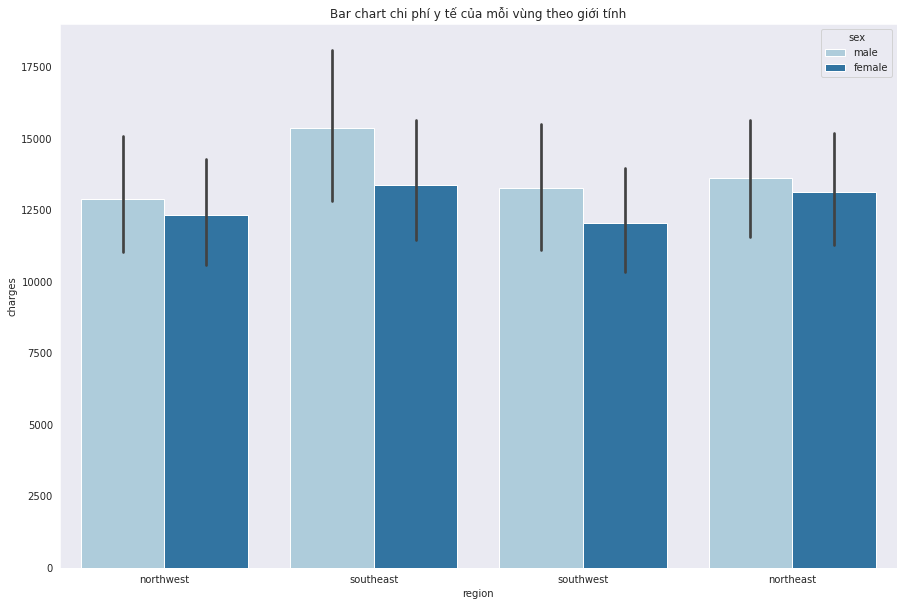
\includegraphics[width=1\textwidth]{images/bar_chart_medical_charges_region_sex.png}
		\caption{Chi phí y tế của mỗi vùng theo giới tính}
		\label{fig:writing-thesis-bar-chart-medical-charges-region-sex}
	\end{figure}
	\textbf{Nhận xét:} 
	\begin{itemize}
		\item Xét chi phí y tế là gần như tương đương nhau. Chi phí y tế của nam giới cao hơn hẳn so với nữ giới, ta có thể suy luận rằng lượng người khám và chữa bệnh là nam giới nhiều hơn nữ giới. Và điều này xảy ra ở mọi khu vực và nổi bật hơn ở Đông Nam và Tây Nam.
		\item Các cột chưa có nhiều sự chênh lệch đáng kể. Do đó, nhóm nhận định rằng đặc trưng \textbf{giới tính} có ít sự ảnh hưởng đến chi phí y tế theo từng vùng.
	\end{itemize}
	
	\subsection{6. Phân tích mối quan hệ chi phí y tế - vùng - tình trạng hút thuốc}
	\qquad Xét đặc trưng tình trạng hút thuốc và sự ảnh hưởng của nó đến chi phí y tế cá nhân theo từng vùng được nhóm trực quan bằng biểu đồ cột dưới đây.
	
	Dữ liệu được chọn là chi phí y tế theo trục tung, trục hoành biểu diễn vùng dân cư, mỗi vùng dân cư gồm hai cột: có - không hút thuốc
	\begin{figure}[H]
		\centering
		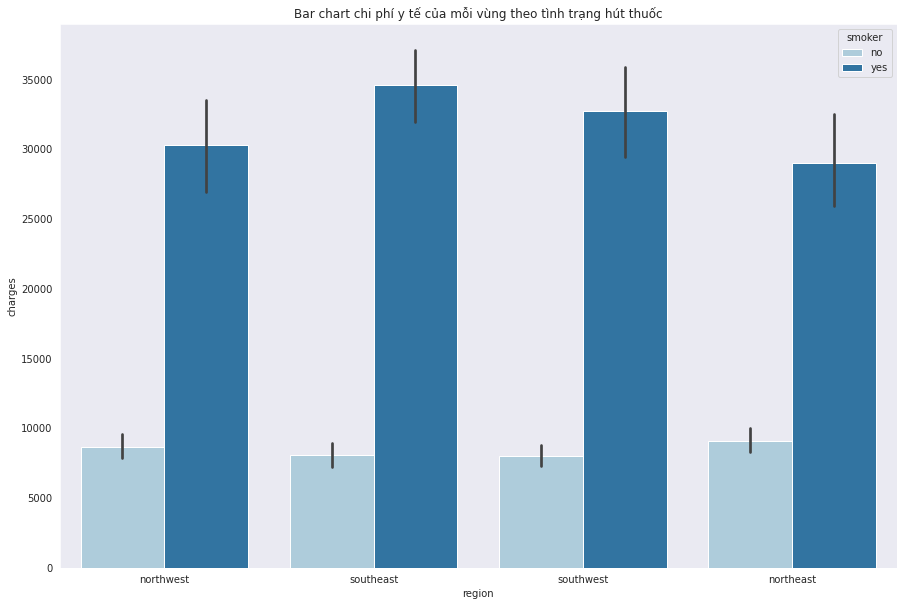
\includegraphics[width=1\textwidth]{images/bar_chart_medical_charges_region_smoker.png}
		\caption{Chi phí y tế của mỗi vùng theo tình trạng hút thuốc}
		\label{fig:writing-thesis-bar-chart-medical-charges-region-smoker}
	\end{figure}
	\textbf{Nhận xét:} 
	\begin{itemize}
		\item Xét ở mỗi vùng dân cư, số lượng người có hút thuốc cao hơn khoảng 3 lần so với người không hút.
		\item Ở khu vực miền Bắc lượng người hút thuốc thấp hơn so với miền Nam.
		\item Đồng thời ở khu vực miền Bắc lượng người không hút thuốc lớn hơn so với miền Nam. => tỉ lệ người không hút thuốc so với hút thuốc ở miền Bắc vượt trội với Miền Nam.
		\item Nhóm nhận định đặc trưng tình trạng hút thuốc là một trong những đặc trưng có sự ảnh hưởng tương đối lớn đối với chi phí y tế cá nhân.
	\end{itemize}

	\subsection{7. Phân tích mối quan hệ chi phí y tế - vùng - số lượng trẻ con/ người phụ thuộc}
	\qquad Xem xét đặc trưng số lượng trẻ con/ người phụ thuộc và sự ảnh hưởng của nó đến chi phí y tế cá nhân theo từng vùng được nhóm trực quan bằng biểu đồ cột dưới đây.
	
	Dữ liệu được chọn là chi phí y tế theo trục tung, trục hoành biểu diễn vùng dân cư, mỗi vùng dân cư gồm sáu cột: 0, 1, 2, 3, 4, 5 tương ứng với số lượng trẻ em/ người phụ thuộc
	\begin{figure}[H]
		\centering
		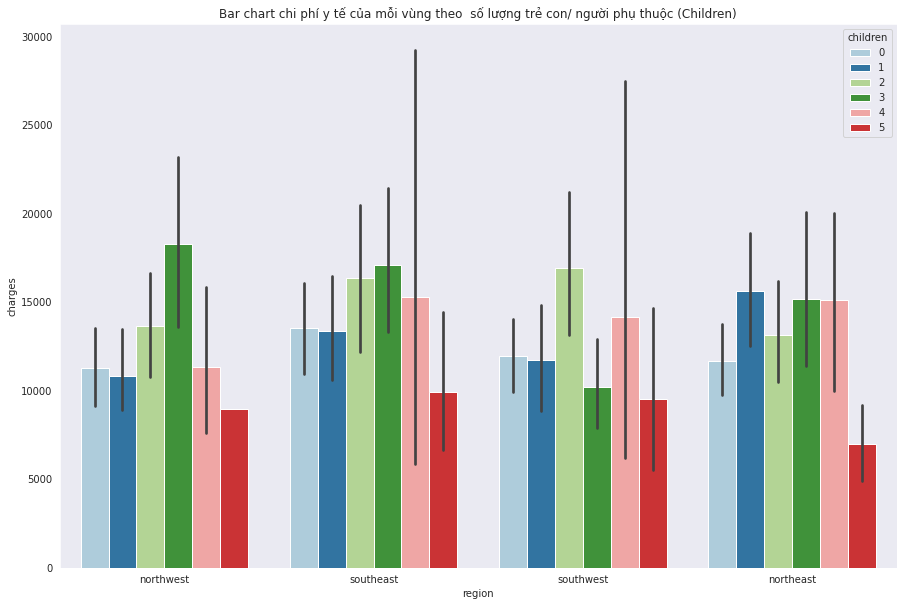
\includegraphics[width=1\textwidth]{images/bar_chart_medical_charges_region_children.png}
		\caption{Chi phí y tế của mỗi vùng theo số lượng trẻ con/ người phụ thuộc}
		\label{fig:writing-thesis-bar-chart-medical-charges-region-children}
	\end{figure}
	\textbf{Nhận xét:} 
	\begin{itemize}
		\item Nhìn chung chi phí y tế cá nhân ở người có 3 đứa trẻ đứng cao ngoại trừ vùng dân cư Tây Nam. 
		\item Chi phí y tế cá nhân ở người có 5 đứa trẻ ở mọi khu vực là thấp nhất. Điều này có nghĩa là ở đất nước này, khi có nhiều trẻ em/ người phụ thuộc người ta thường phải chi tiêu chặt chẽ hơn, tầng lớp người này có thể là người thu nhập trung bình khá, trung bình, nghèo do đó điều kiện không cho phép họ chi quá nhiều vào Y tế.
		\item Chi phí y tế cá nhân ở người không có trẻ em/ người phụ thuộc tương đối cao, cao hơn mức những người có 5 đứa trẻ/ người phụ thuộc.
		\item Nhóm nhận định đặc trưng số lượng trẻ con/ người phụ thuộc là một đặc trưng có ảnh hưởng tương đối ít đối với chi phí y tế cá nhân.
	\end{itemize}
	
	\subsection{8. Phân tích mối quan hệ giữa chi phí y tế và tuổi nhóm theo tình trạng hút thuốc}
	\qquad Xem xét mô hình tuyến tính (Linear Model) giữa  chi phí y tế và tuổi nhóm theo tình trạng hút thuốc
	
	Do hai đặc trưng chi phí y tế và tuổi là hai đại lượng liên tục nên dùng biểu đồ linear model trực quan quan hệ giữa chúng.
	
	Việc phân lớp theo đặc trưng tình trạng hút thuốc do đặc trưng này được nhóm nhận định là có ảnh hưởng khá lớn đối với chi phí y tế cá nhân
	\begin{figure}[H]
		\centering
		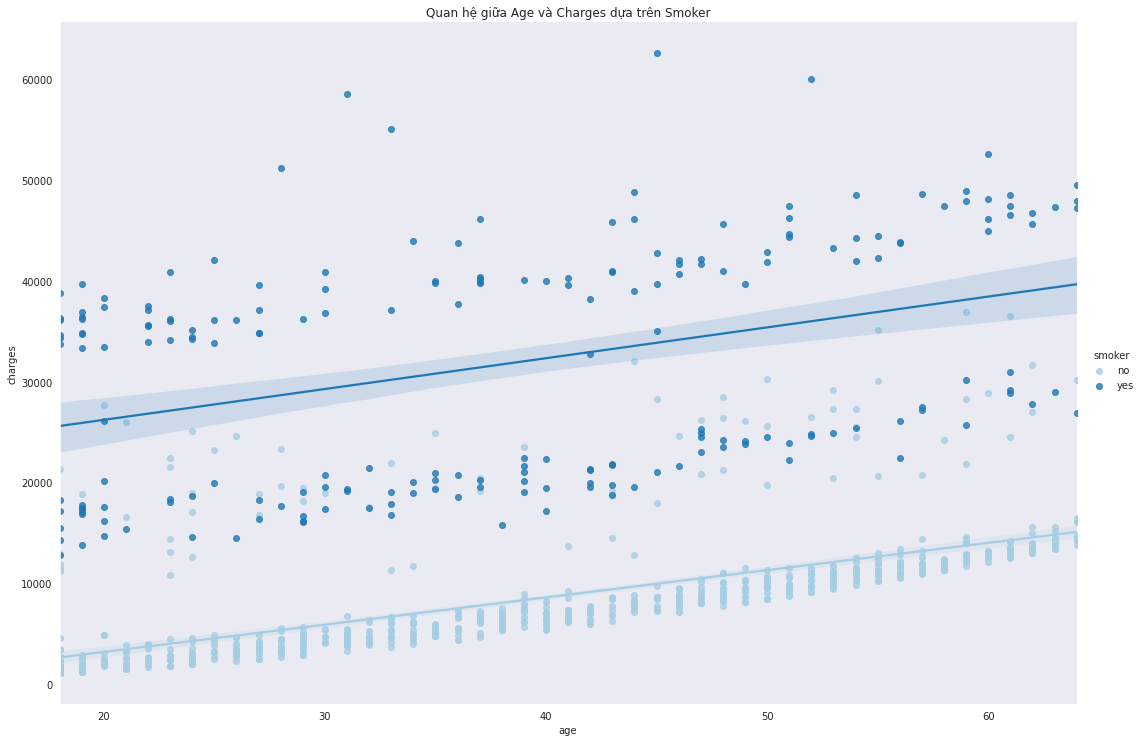
\includegraphics[width=1\textwidth]{images/age_charges_by_smoker.png}
		\caption{Quan hệ giữa Age và Charges dựa trên Smoker}
		\label{fig:writing-thesis-linear-model-medical-charges-age-group-smoker}
	\end{figure}
	\textbf{Nhận xét:} 
	\begin{itemize}
		\item Chi phí y tế của người hút thuốc cao hơn so với người không hút thuốc khoảng 23000.
		\item Chi phí y tế sẽ tăng dần đều theo số tuổi của người bệnh dù có hút thuốc hay không. => số tiền viện phí tăng thêm cần bỏ ra khi khám phụ thuộc vào tuổi, hút thuốc sẽ tăng thêm số tiền cố định thay vì tỉ lệ tăng dần.
	\end{itemize}

	\subsection{9. Phân tích mối quan hệ giữa chi phí y tế và chỉ số BMI nhóm theo tình trạng hút thuốc}
	\qquad Xem xét mô hình tuyến tính (Linear Model) giữa  chi phí y tế và chỉ số BM nhóm theo tình trạng hút thuốc
	
	Do hai đặc trưng chi phí y tế và chỉ số BM là hai đại lượng liên tục nên dùng biểu đồ linear model trực quan quan hệ giữa chúng.
	
	Việc phân lớp theo đặc trưng tình trạng hút thuốc do đặc trưng này được nhóm nhận định là có ảnh hưởng khá lớn đối với chi phí y tế cá nhân
	\begin{figure}[H]
		\centering
		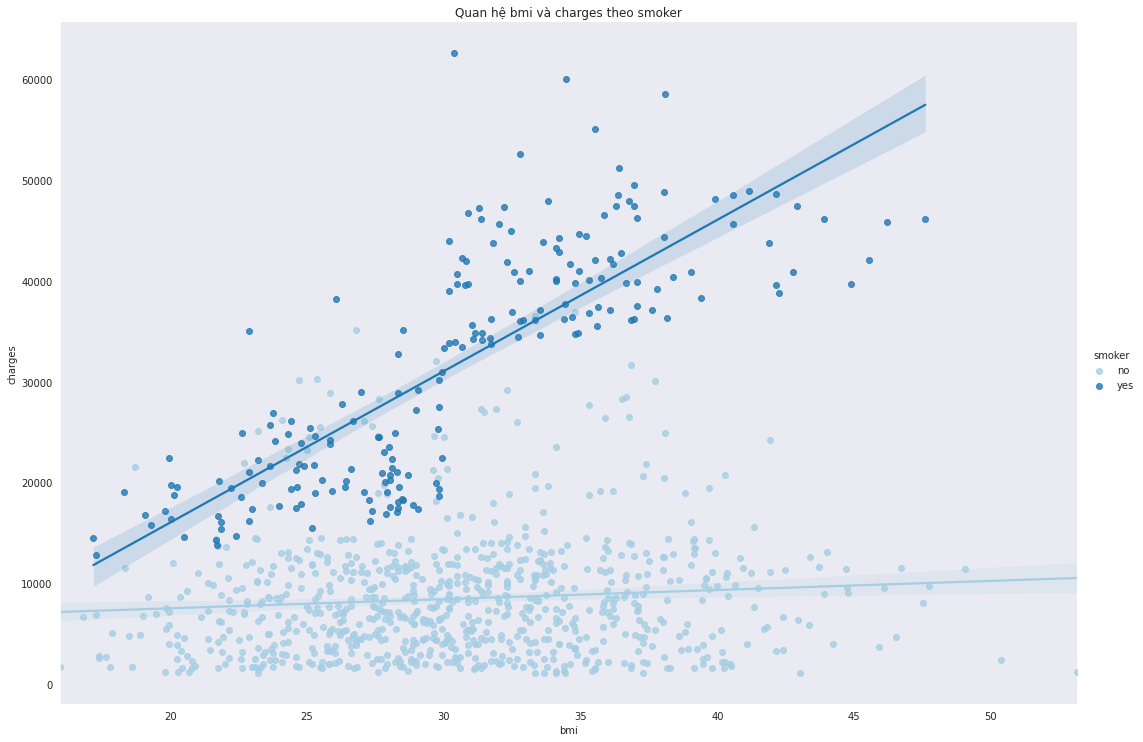
\includegraphics[width=1\textwidth]{images/bmi_charges_by_smoker.png}
		\caption{Quan hệ giữa Bmi và Charges dựa trên Smoker}
		\label{fig:writing-thesis-linear-model-medical-charges-bmi-group-smoker}
	\end{figure}
	\textbf{Nhận xét:} 
	\begin{itemize}
		\item Biểu đồ cho ta thấy số tiền viện phí khi không hút thuốc sẽ ổn định bất kể số bmi.
		\item Chi phí y tế của người không hút thuốc tăng với tỉ lệ cực thấp nếu không hút thuốc.
		\item Chi phí y tế của người hút thuốc sẽ tăng cao tỉ lệ thuận với bmi.
		\item Ở người hút thuốc tỉ lệ người có bmi thấp cao hơn so với ở người không hút.
	\end{itemize}

	\subsection{10. Phân tích  mối quan hệ giữa chi phí y tế và số lượng trẻ con/ người phụ thuộc nhóm theo tình trạng hút thuốc}
	\qquad Xem xét mô hình tuyến tính (Linear Model) giữa  chi phí y tế và số lượng trẻ con/ người phụ thuộc nhóm theo tình trạng hút thuốc
	
	Do hai đặc trưng chi phí y tế và số lượng trẻ con/ người phụ thuộc là hai đại lượng liên tục nên dùng biểu đồ linear model trực quan quan hệ giữa chúng.
	
	Việc phân lớp theo đặc trưng tình trạng hút thuốc do đặc trưng này được nhóm nhận định là có ảnh hưởng khá lớn đối với chi phí y tế cá nhân
	\begin{figure}[H]
		\centering
		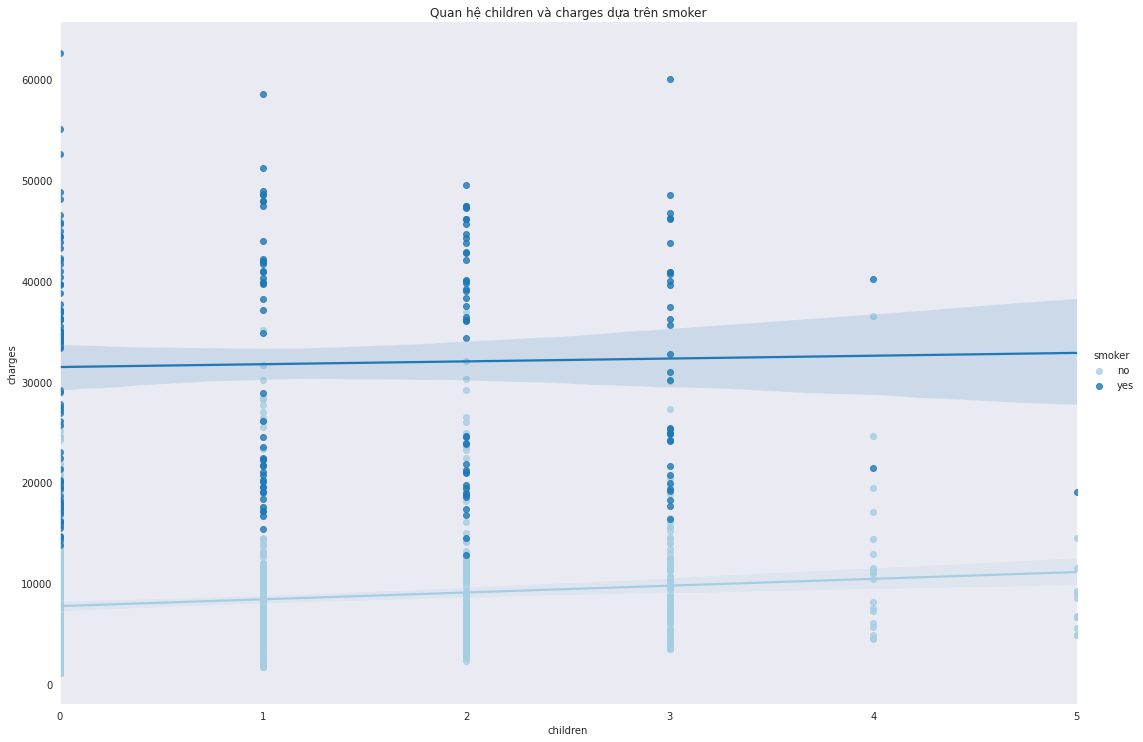
\includegraphics[width=1\textwidth]{images/children_charges_by_smoker.png}
		\caption{Quan hệ giữa Children và Charges dựa trên Smoker}
		\label{fig:writing-thesis-linear-model-medical-charges-children-group-smoker}
	\end{figure}
	\textbf{Nhận xét:} 
	\begin{itemize}
		\item
	\end{itemize}

	\subsection{11. Kết luận - Suy diễn}
	
	\section{3. Cài đặt thuật toán Máy học}
	
	\subsection{1. Lựa chọn thuật toán Máy học}
	\qquad Vấn đề đặt ra, dựa trên những dự kiện (các biến, giả định rằng các biến này độc lập với nhau) về tuổi (age), giới tính (sex), bmi, số lượng trẻ em (children), vùng dân cư (region), ta có thể đưa ra dự đoán về giá trị của chi phí y tế cá nhân (biến phụ thuộc) một cách chính xác nhất có thể
	
	Đây là một bài toán có thể áp dụng Mô hình Tuyến tính và Phân tích Hồi quy
	
	\textbf{Nhắc lại về bài toán Phân tích Hồi quy}
	Giả sử rằng một kết quả một quá trình bất kỳ nào đó được đại diện bằng một biến ngẫu nhiên $Y$, $Y$ được gọi là biến phụ thuộc, phụ thuộc vào $k$ biến khác $X_1, X_2, ..., X_k$

	Giả sử, biến $Y$ có thể được biểu diễn dạng như sau:
	\begin{align*}
		Y = f(X_1, X_2, ..., X_k, \beta_1, \beta_2, ..., \beta_k) + \beta_0
	\end{align*}
	Hàm $f$ là một hàm lý tưởng, $\beta_1, \beta_2, ..., \beta_k$ thể hiện sự đóng góp của $X_1, X_2, ..., X_k$, giá trị $\beta_0$ thể hiện sự ngẫu nhiên giữa $Y$ với $X_1, X_2, ..., X_k$
	
	Mô hình hay quan hệ này được gọi là tuyến tính nếu nó tuyến tính với các tham số của nó và phi tuyến nếu nó không tuyến tính với các tham số của nó. Có nghĩa là, nếu tất cả đạo hàm $y$ theo từng biến tham số $\beta_1, \beta_2, ..., \beta_k$ độc lập với các tham số thì mô hình gọi là tuyến tính.
	
	\textbf{Các bước thực hiện của Phân tích Hồi quy}
	\begin{itemize}
		\item Phát biểu bài toán/ vấn đề
		\item Lựa chọn những biến có liên quan đến bài toán
		\item Thu thập dữ liệu về những biến đã chọn có liên quan đến bài toán
		\item Đặc điểm kỹ thuật của mô hình
		\item Lựa chọn phương pháp để điều chỉnh dữ liệu
		\item Khớp mô hình
		\item Kiểm định và đánh giá mô hình
		\item Sử dụng (các) mô hình đã chọn cho giải pháp của vấn đề đã đặt ra.
	\end{itemize}

	\textbf{Mục tiêu của Phân tích Hồi quy} Việc xác định dạng tường minh của phương trình hồi quy là mục tiêu cuối cùng của phân tích hồi quy. Cuối cùng nó là một mối quan hệ tốt và hợp lệ giữa biến nghiên cứu và biến giải thích. Một phương trình hồi quy như vậy có thể được sử dụng cho một số mục đích. 
	
	Ví dụ, để xác định vai trò của bất kỳ biến giải thích nào trong mối quan hệ chung trong bất kỳ xây dựng chính sách nào, để dự báo các giá trị của biến phản hồi cho một tập hợp các giá trị nhất định của các biến giải thích. Phương trình hồi quy giúp hiểu được mối quan hệ qua lại của các biến giữa chúng.
	
	\subsection{2. Hồi quy Tuyến tính - Linear Regression}
	\subsubsection{Hồi quy tuyến tính cơ bản}
	\subsubsection{Sklearn Hồi quy tuyến tính}
	
	\subsection{3. Hồi quy Ridge - Ridge Regression}
	\subsubsection{Hồi quy Ridge cơ bản}
	\subsubsection{Sklearn Hồi quy Ridge}
	\subsection{4. Hồi quy Lasso - Lasso Regression}
	\subsubsection{Hồi quy Lasso cơ bản}
	\subsubsection{Sklearn Hồi quy Lasso}
	\subsection{5. Hồi quy rừng ngẫu nhiên - Random Forest Regressor}
	\subsubsection{Hồi quy rừng ngẫu nhiên cơ bản}
	\subsubsection{Sklearn Hồi quy rừng ngẫu nhiên}
	\subsection{6. Hồi quy đa thức - Polynomial Regression}
	\subsubsection{Hồi quy đa thức cơ bản}
	\subsubsection{Sklearn Hồi quy đa thức}
	\section{4. Các kết quả và nhận xét}
	
	\nocite{*}
	\bibliography{references}\newpage\cleardoublepage
	\bibliographystyle{plain}
	
\end{document}